Due to our limitation in computing resources, we can only present our approaches for the first 30 bins (meaning videos with age ranging from 1 day to 30 days). For each bin, we create 5 folds cross-validation with 80\% of our data for training, and the other 20\% for testing. The average results over 5-folds are reported.

\subsubsection{Classification Results}
	The results of our logistic regression comparing paris of videos are
	
	
\subsubsection{Regression Results}
	The linear regression can be evaluated in more than one way.
	
	The first way to measure our results is to look at its predictions directly.  Our mean squared error indicated that our prediction was was typically 0.93 orders of magnitude away from the true result, but it is hard to say whether we should be impressed.
	
	The second form of evaluation is to compare the results for each pair of videos and then use the \textbf{0-1 loss function}, so that results can be compared to the logistic regression results.  Not surprisingly, logistic regression performed better (having been trained explicitly for this task).  What is surprising, however, is that our accuracy is not significantly greater than 50\%, which indicates that our linear regression holds no measurable value for the ranking problem.
	
	A likely cause is that this problem may not be linear in nature -- in fact, it would admittedly be surprising if it were.  We tested our accuracy on the training data as well as on the testing data, and found that it performed just as poorly, indicating that the weak results on our testing data did not stem from over fitting.
	
	In order to investigate further, we plotted our output against the true number of views (for a random subset of our data):

	\begin{figure}[!h]
		\begin{center}
			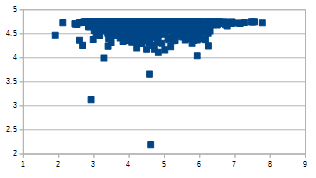
\includegraphics[width=.75\textwidth,clip]{logistic regression training.png}
		\end{center}
		\caption{Training data: true value vs prediction (in log-scale).}
		\label{fig:trainingTrueVsPredicted}
	\end{figure}
	
	\begin{figure}[!h]
		\begin{center}
			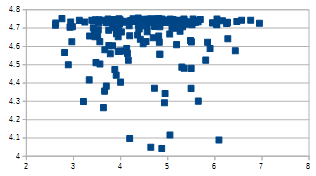
\includegraphics[width=.75\textwidth,clip]{logistic regression testing.png}
		\end{center}
		\caption{Testing data: true value vs prediction (in log-scale).}
		\label{fig:testingTrueVsPredicted}
	\end{figure}
	
	We observe a strong tendency towards the same output value (roughly 50,000 views), which corresponds to the average number of views -- this would be the typical outcome when linear regression is inadequate.
